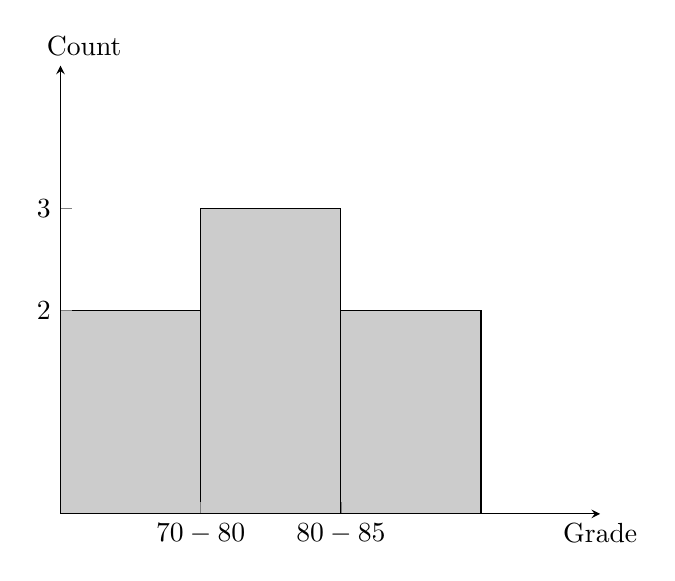
\begin{tikzpicture}
\begin{axis}[
no markers,
axis lines*=center,
enlargelimits = upper, clip=true,
ylabel={Count},
xlabel={Grade},
axis on top,
axis line style={->,>=stealth},
every axis x label/.style={
	at={(ticklabel* cs:1)},
	anchor=north,
},
every axis y label/.style={
	at={(ticklabel* cs:1)},
	anchor=south,
	xshift=0.3cm,
},
ymin=0, ymax=4,
xmin=1, xmax=4.5,
ytick={0, 2, 3},
xtick={1,...,3},
xticklabels={$<70$, $70-80$, $80-85$, $85-90$},
]
\addplot[black, ybar interval, fill=black!20, mark=no] plot coordinates {(1, 2) (2, 3) (3, 2) (4, 3)};
\end{axis}
\end{tikzpicture}